\documentclass[tikz,border=5pt]{standalone}
\usepackage{pgfplots}
\pgfplotsset{compat=1.17}
\usetikzlibrary{decorations.pathreplacing,arrows.meta}

% Custom colors
\definecolor{lila}{RGB}{152,78,163}
\definecolor{amarillo}{RGB}{255,127,0}

\begin{document}
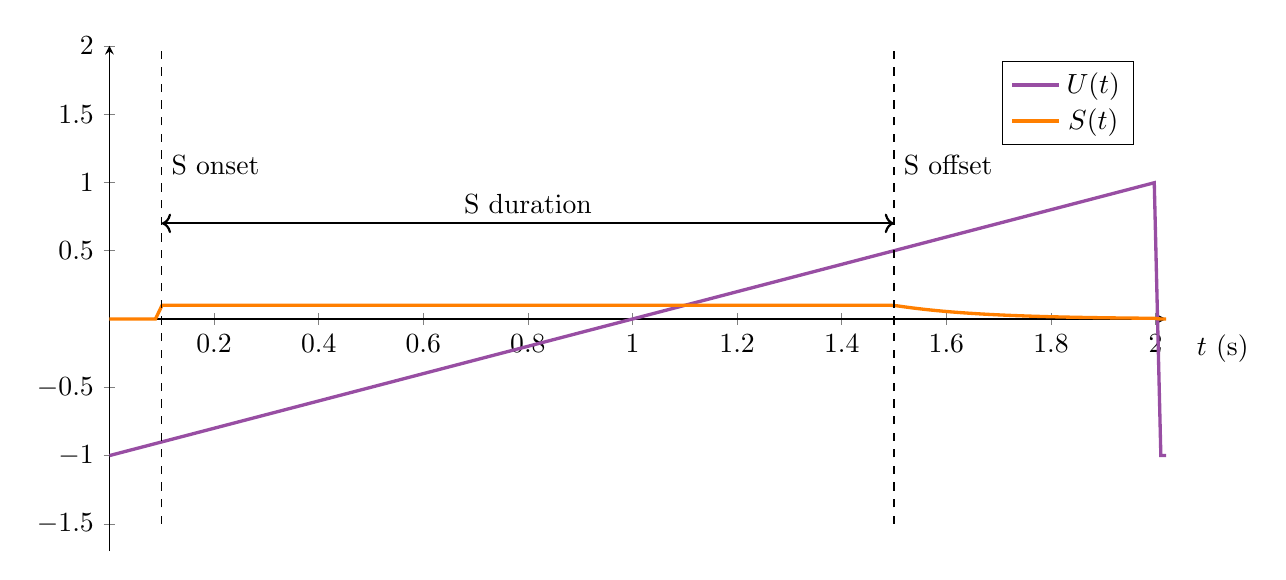
\begin{tikzpicture}

% Parameter definitions
\pgfmathsetmacro{\Uonset}{0}
\pgfmathsetmacro{\Uoffset}{2}
\pgfmathsetmacro{\Uamp}{2}

\pgfmathsetmacro{\Sonset}{0.1}
\pgfmathsetmacro{\SD}{1.4}      % stimulus duration = offset - onset = 1.7-0.3
\pgfmathsetmacro{\Sd}{0.5}      % decay time constant for tail
\pgfmathsetmacro{\Samp}{0.1}

\begin{axis}[
  width=15cm, height=8cm,
  domain=0:2.5, samples=200,
  xmin=0, xmax=2.02,
  ymin=-1.7, ymax=2.0,
  axis lines=middle,
  xlabel={$t\ (\mathrm{s})$}, ylabel={},
  legend pos=north east,
  every axis x label/.style={at={(axis description cs:1.02,0.40)},anchor=west},
  every axis y label/.style={at={(axis description cs:0.05,0.90)},anchor=south},
]

% Plot U(t)
\addplot[lila, very thick] 
  ( {x}, 
    { x<\Uonset || x>\Uoffset 
      ? -1 
      : -1 + \Uamp*(x-\Uonset)/(\Uoffset-\Uonset) }
  );
\addlegendentry{$U(t)$}

% Plot S(t)
\addplot[amarillo, very thick]
  ( {x},
    { x<\Sonset || x>(\Sonset+\SD+\Sd)
      ? 0
      : ( x<=\Sonset+\SD 
          ? \Samp 
          : \Samp*exp(-3*(x-(\Sonset+\SD))/\Sd)
        )
    }
  );
\addlegendentry{$S(t)$}

\draw[dashed] (axis cs:\Sonset,-1.5) -- (axis cs:\Sonset,2)
   node[right, pos = 3/4] {S onset};


\draw[<->,thick]
  (axis cs:\Sonset,0.7) -- node[above] {S duration}
  (axis cs:{\Sonset+\SD},0.7);
  
\draw[dashed] (axis cs:\Sonset+\SD,-1.5) -- (axis cs:\Sonset+\SD,2)
   node[right, pos = 3/4] {S offset};


\end{axis}
\end{tikzpicture}
\end{document}
